\documentclass{beamer}

\usepackage[czech]{babel}
\usepackage[utf8]{inputenc}
\usepackage[T1]{fontenc}
\usepackage{lmodern}
\usepackage{datetime}
\usepackage{tikz}
\usepackage{amssymb}
\usepackage{bbding}
\usepackage{tabularx}
\usepackage{wrapfig}
\usepackage{xcolor}

\usetikzlibrary{shadows}

\definecolor{sourcesclr}{rgb}{.38,.38,.38}

% Themes: http://www.hartwork.org/beamer-theme-matrix/
\mode<presentation>{\usetheme{Madrid}}
\usecolortheme{default}
\beamertemplatenavigationsymbolsempty 
\setbeamertemplate{title page}[default][colsep=0bp,rounded=true]
\setbeamertemplate{itemize items}{$\star$}
\setbeamercolor*{item}{fg=black}
\setbeamertemplate{enumerate item}[default]
\newcommand{\Has}{\textcolor{green}{\CheckmarkBold}}
\newcommand{\NoHas}{\textcolor{red}{\XSolidBrush}}
\newcommand{\It}{\textit}  % kurzíva
\newcommand{\B}{\textbf} %tučné písmo
\newcommand{\U}{\underline}  % podtržené písmo
\newcommand{\sectsel}[1]{\U{\B{#1}}}
\newcommand{\srctext}[1]{{\fontsize{7}{9}\selectfont\textcolor{sourcesclr}{#1}}}

\newenvironment<>{positiveblock}[1]{%
  \begin{actionenv}#2%
      \def\insertblocktitle{#1}%
      \par%
      \mode<presentation>{%
        \setbeamercolor{block title}{fg=white,bg=green!20!black}
       \setbeamercolor{block body}{fg=black,bg=green!40}
       \setbeamercolor{itemize item}{fg=green!20!black}
       \setbeamertemplate{itemize item}[triangle]
     }%
      \usebeamertemplate{block begin}}
    {\par\usebeamertemplate{block end}\end{actionenv}}

\newenvironment<>{negativeblock}[1]{%
  \begin{actionenv}#2%
      \def\insertblocktitle{#1}%
      \par%
      \mode<presentation>{%
        \setbeamercolor{block title}{fg=white,bg=red!20!black}
       \setbeamercolor{block body}{fg=black,bg=red!20}
       \setbeamercolor{itemize item}{fg=red!20!black}
       \setbeamertemplate{itemize item}[triangle]
     }%
      \usebeamertemplate{block begin}}
    {\par\usebeamertemplate{block end}\end{actionenv}}

\author{Vojtěch Boček}
\institute[vbocek@gmail.com]{SPŠ a VOŠ technická Brno, Sokolská 1}
\title{MultiROM}
\subtitle{Nástroj pro instalaci více operačních systémů\\na jedno mobilní zařízení}
\date[]{}

\setbeamerfont{sections}{size=\fontsize{8}{9}\selectfont}

\begin{document}


\frame{\titlepage}

\begin{frame}
    \begin{center}
        \vspace{15mm}
        \begin{figure}[H]
        
\includegraphics[width=120px]{../img/broken_android.png}
        \end{figure}
    \end{center}
    \vspace{20mm}
    \srctext{Zdroj obrázku: android / platform/bootable/recovery@280a238b / res/icon{\textunderscore}error.png}
\end{frame}

\begin{frame}
    \frametitle{MultiROM}
    \begin{columns}
    \column{.48\textwidth}
    \vspace{-10mm}
    \begin{itemize}
        \item instalace libovolného množství vedlejších systémů -- \It{multiboot}
        \item podpora mnoha operačních systémů
        \item snadné používání
    \end{itemize}
    \column{.48\textwidth}
    \vspace{-5mm}
    \begin{figure}[H]
    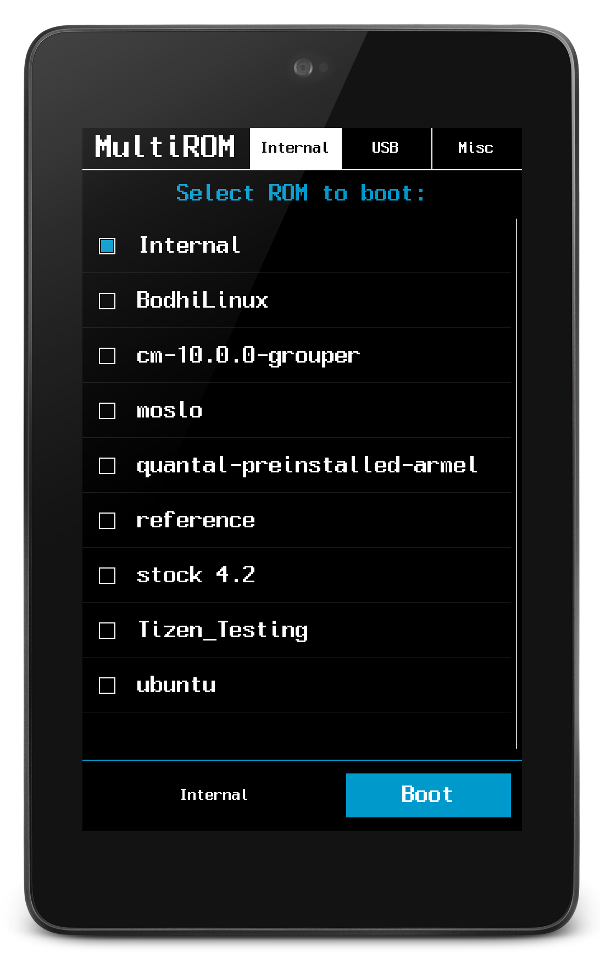
\includegraphics[width=145px]{../img/boot_manager_promo.png}
    \end{figure}
%     \begin{figure}[H]
%     \begin{tikzpicture}
%         \node[drop shadow={shadow xshift=.8ex,shadow yshift=-.8ex},fill=white,draw] at (0,0) { 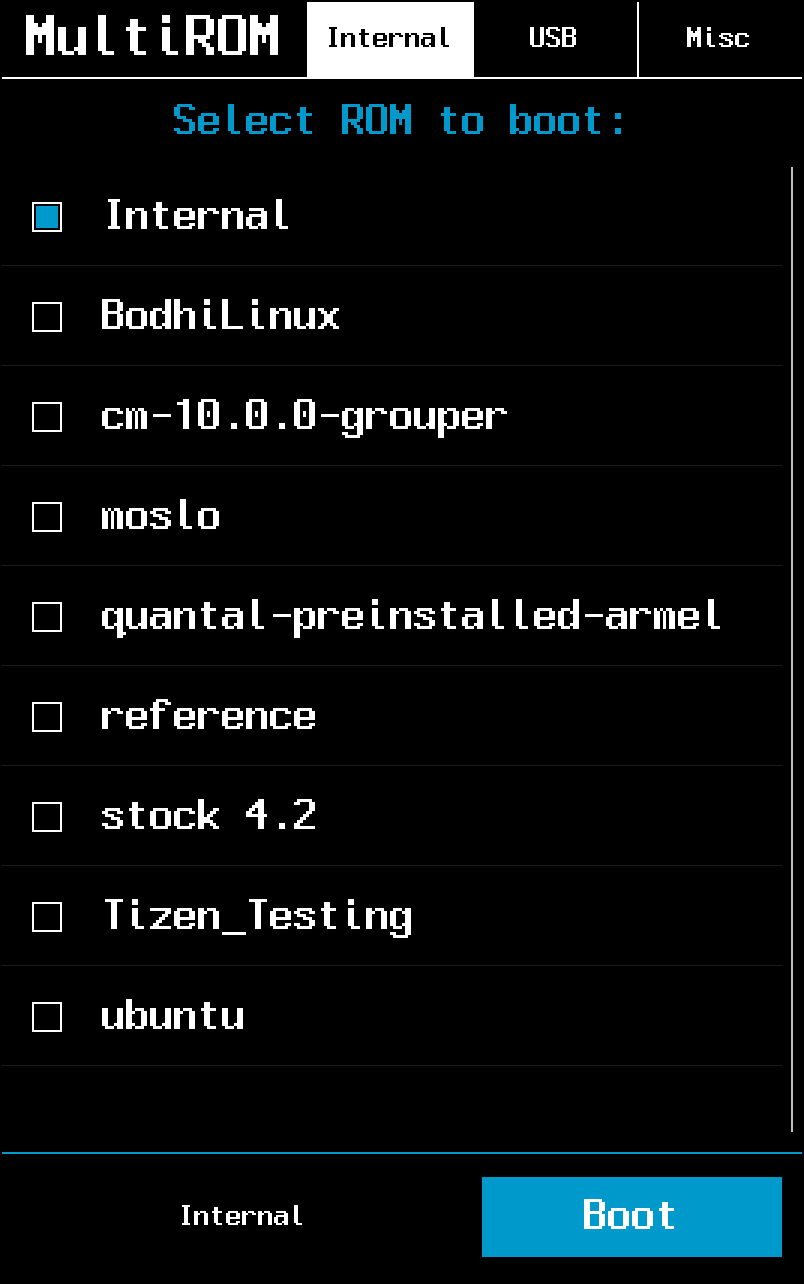
\includegraphics[width=120px]{../img/boot_manager.png}};
%     \end{tikzpicture}
%     \end{figure}
    \end{columns}
\end{frame}


\begin{frame}
    \frametitle{Aktuální stav}
    \begin{itemize}
        \item oficiálně podporována 4 zařízení (tablety Nexus 7 2012 \& 2013 a telefony Nexus 4 a Nexus 5)
        \pause
        \item více než desítka dalších zařízení podporována komunitou
        \pause
        \item úspěšný crowdfunding projekt
        \pause
        % Z jakých států a tak
        \item přes 18 000 aktivních instalací
    \end{itemize}
    \begin{figure}[H]
    \begin{tikzpicture}
         \node[fill=white,draw] at (0,0) { 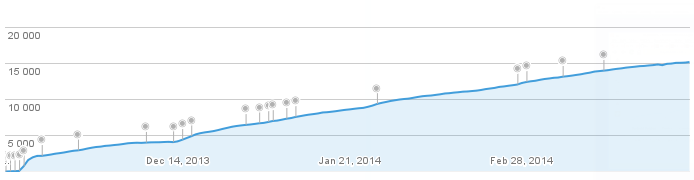
\includegraphics[width=0.95\textwidth]{../img/graph_active.png}};
    \end{tikzpicture}
    \end{figure}
    \vspace{-5mm}
    \hspace{1mm} \srctext{Zdroj: Google Play Store statistiky pro vývojáře}
\end{frame}

% \begin{frame}
%     \frametitle{Části projektu}
%     \begin{enumerate}
%         \item Boot manager
%         \item Upravená recovery
%         \item Kexec-hardboot patch
%         \item Aplikace pro Android
%     \end{enumerate}
% \end{frame}

\begin{frame}
    \vspace{-2.5ex}
    \begin{beamercolorbox}[wd=\paperwidth,ht=2.5ex,dp=1.125ex,center=true]{palette quaternary}%
    \usebeamerfont{sections}
    \sectsel{1. Boot manager} | 2. Upravená recovery | 3. Kexec-hardboot patch | 4. Aplikace pro Android
    \end{beamercolorbox}
    \vspace{-1.5ex}

    \frametitle{Boot Manager}
    \begin{columns}
    \column{.48\textwidth}
    \begin{itemize}
        \item zobrazuje se po spuštění zařízení
        \item slouží pro výběr systému
        \item obsahuje kód, který se stará o multiboot
        \item umí automaticky spustit nastavený systém
    \end{itemize}
    \vspace{10mm}

    \column{.48\textwidth}
    \begin{figure}[H]
    \begin{tikzpicture}
        \node[drop shadow={shadow xshift=.8ex,shadow yshift=-.8ex},fill=white,draw] at (0,0) { 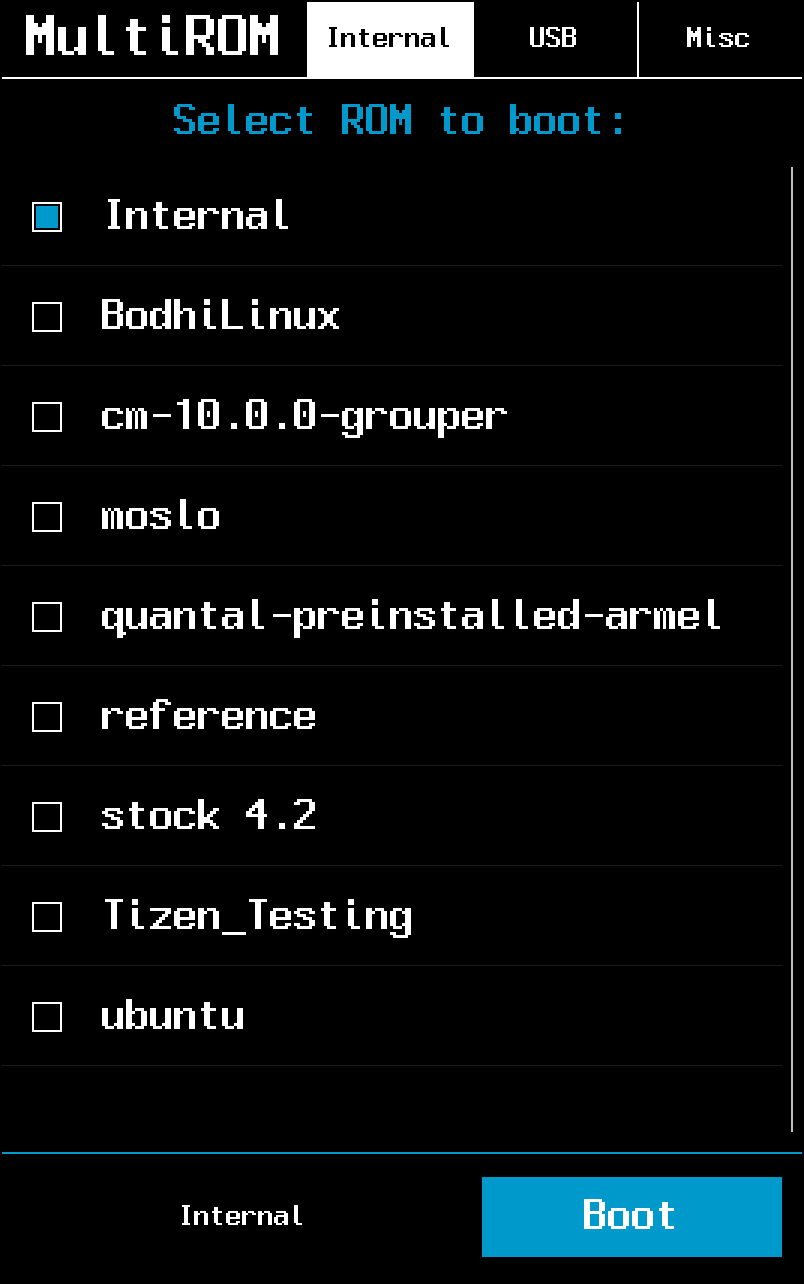
\includegraphics[width=120px]{../img/boot_manager.png}};
    \end{tikzpicture}
    \end{figure}
    \end{columns}
\end{frame}

\begin{frame}
    \vspace{-2.0ex}
    \begin{beamercolorbox}[wd=\paperwidth,ht=2.5ex,dp=1.125ex,center=true]{palette quaternary}%
    \usebeamerfont{sections}
    1. Boot manager | \sectsel{2. Upravená recovery} | 3. Kexec-hardboot patch | 4. Aplikace pro Android
    \end{beamercolorbox}
    \vspace{-1.5ex}

    \frametitle{Upravená recovery}
    \begin{columns}
    \column{.48\textwidth}
    \begin{itemize}
        \item původně zejména pro opravu hlavního systému
        \item správa vedlejších systémů
        \item nastavení MultiROM
        \item založená na open-source projektu TWRP
    \end{itemize}
    \vspace{10mm}

    \column{.48\textwidth}
    \begin{figure}[H]
    \begin{tikzpicture}
        \node[drop shadow={shadow xshift=.8ex,shadow yshift=-.8ex},fill=white,draw] at (0,0) { 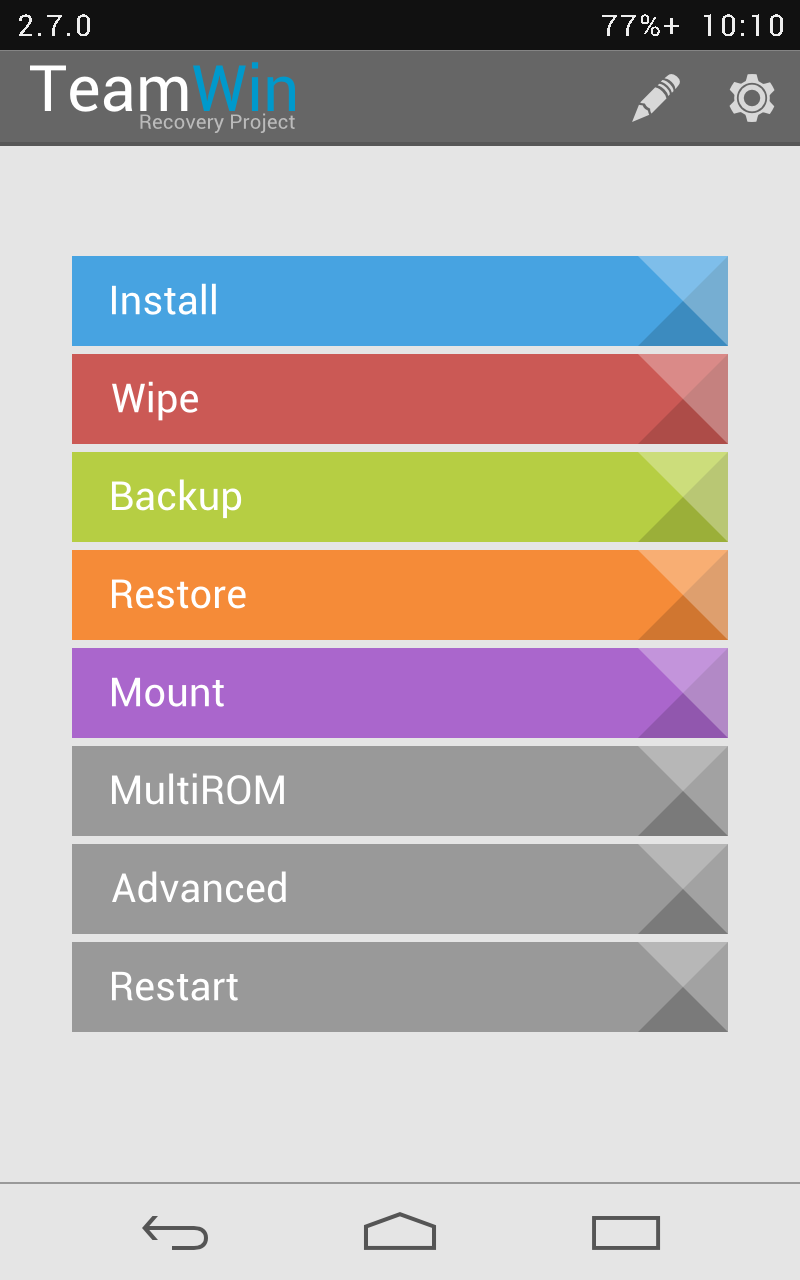
\includegraphics[width=120px]{../img/recovery2.png}};
    \end{tikzpicture}
    \end{figure}
    \end{columns}
\end{frame}

\begin{frame}
    \vspace{-12.4ex}
    \begin{beamercolorbox}[wd=\paperwidth,ht=2.5ex,dp=1.125ex,center=true]{palette quaternary}%
    \usebeamerfont{sections}
    1. Boot manager | 2. Upravená recovery | \sectsel{3. Kexec-hardboot patch} | 4. Aplikace pro Android
    \end{beamercolorbox}
    \vspace{13.0ex}

    \frametitle{Kexec-hardboot patch}
    \begin{itemize}
        \item úprava Linuxového jádra
        \item spouštění jiného jádra s pomocí toho již běžícího
        %\item nepřepíše jádro uložené v boot sektoru
        \item \B{technicky umožňuje multiboot na zařízeních s tak limitovaným přístupem, jako jsou tablety a telefony s OS Android}
    \end{itemize}
\end{frame}

\begin{frame}
    \vspace{-3.7ex}
    \begin{beamercolorbox}[wd=\paperwidth,ht=2.5ex,dp=1.125ex,center=true]{palette quaternary}%
    \usebeamerfont{sections}
    1. Boot manager | 2. Upravená recovery | 3. Kexec-hardboot patch | \sectsel{4. Aplikace pro Android}
    \end{beamercolorbox}
    \vspace{-1.0ex}

    \frametitle{Aplikace pro Android}
    \begin{columns}
    \column{.48\textwidth}
    \begin{itemize}
        \item instalace a aktualizace MultiROM
        \item přejmenovávání a mazání nainstalovaných systémů
        \item bootování přímo do nainstalovaných systémů
    \end{itemize}
    \vspace{10mm}

    \column{.48\textwidth}
    \begin{figure}[H]
    \begin{tikzpicture}
        \node[drop shadow={shadow xshift=.8ex,shadow yshift=-.8ex},fill=white,draw] at (0,0) { 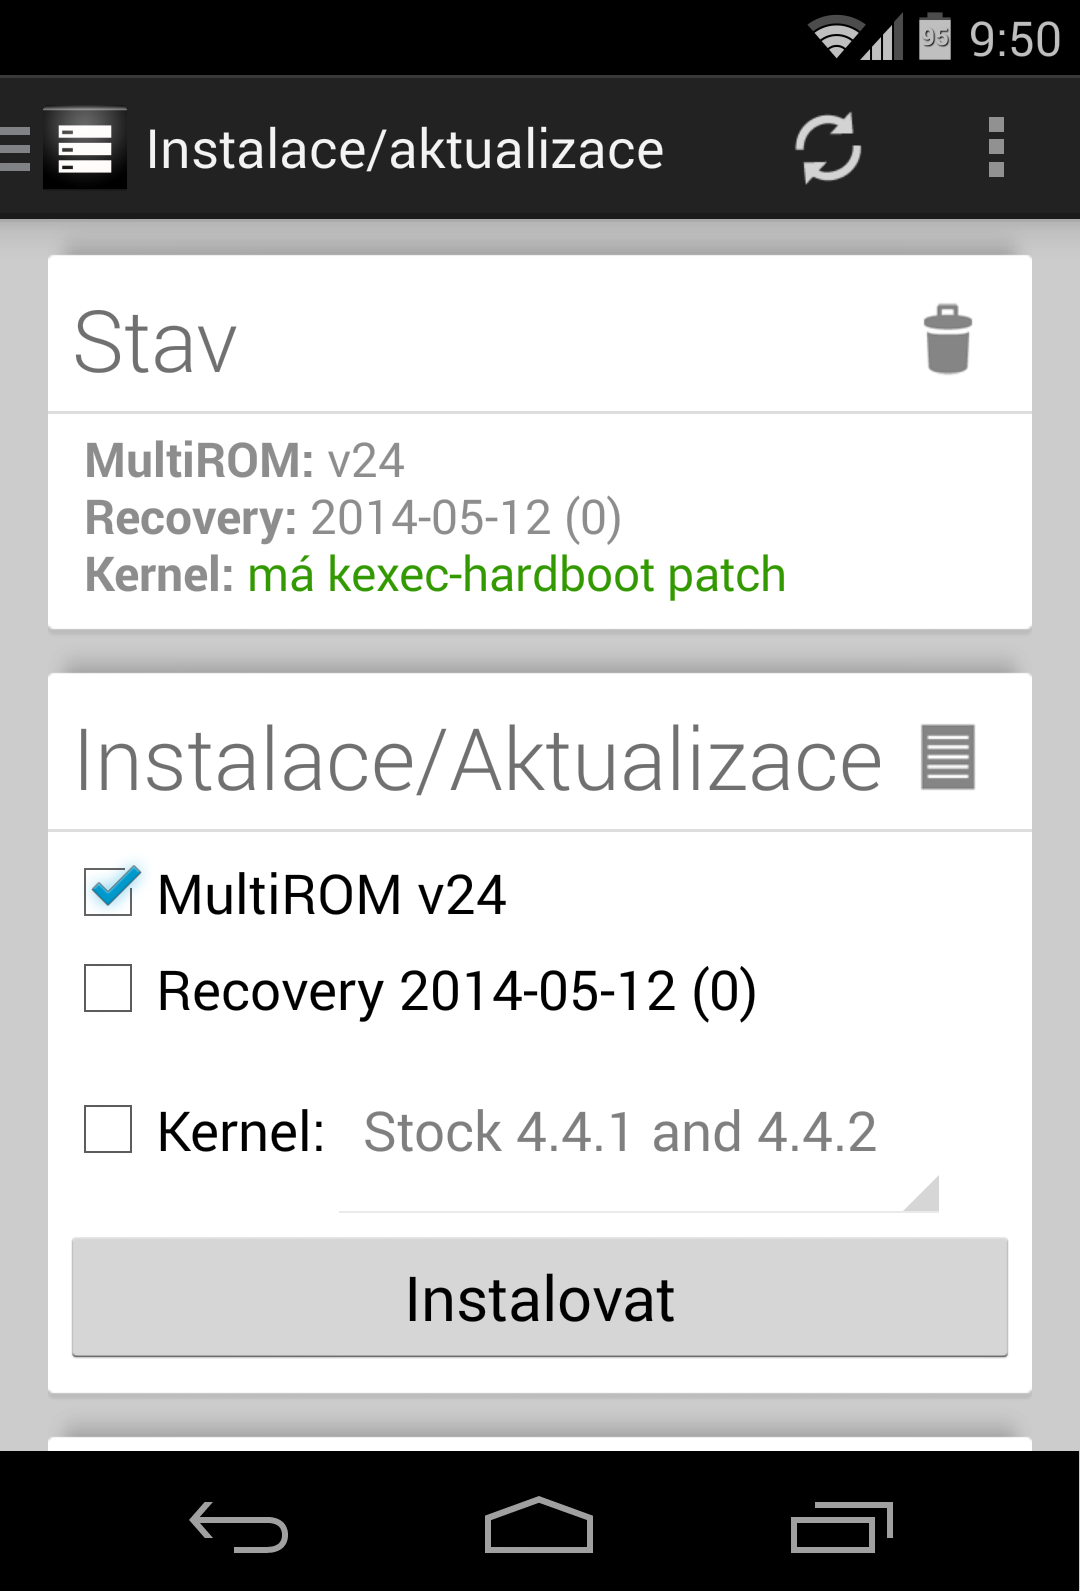
\includegraphics[width=120px]{../img/app_main2.png}};
    \end{tikzpicture}
    \end{figure}
    \end{columns}
\end{frame}

% BOOT MENUp
% to stejne na N5, tam boot android
% N7 - recovery, boot android
% n5 - ukazat nabootovanou rom, reboot do ubuntu
% n7 - ukazat app a widget
% n5 - ukazat ubuntu

\begin{frame}
    \begin{center}
        {\Large *\It{Pravděpodobně} živá ukázka!* }
        \vspace{5mm}
        \begin{figure}[H]
        
\includegraphics[width=0.4\textwidth]{../img/kocka.png}
        \end{figure}
    \end{center}
    \vspace{15mm}
    \srctext{Autor obrázku: Ketrina Yim (draguunthor.deviantart.com)}
\end{frame}


% \begin{frame}
%     \frametitle{Porovnání s existujicími řešeními}
%     \begin{positiveblock}{Výhody}
%     \begin{itemize}
%         \item Velmi snadné používání
%         \item Libovolné množství systémů
%         \item Libovolný typ systémů
%         \item Instalace vedlejších systémů do vnitřní paměti nebo na USB flash disk
%         \item Žádný dopad na rychlost systému
%     \end{itemize}
%     \end{positiveblock}
% 
%     \pause
%     \begin{negativeblock}{Nevýhody}
%     \begin{itemize}
%         \item Nemožnost sdílení aplikací mezi systémy
%     \end{itemize}
%     \end{negativeblock}
% \end{frame}

\begin{frame}
    \frametitle{Proč?}
    \begin{itemize}
        \item na PC je multiboot běžná funkce
        \item vyzkoušení jiných operačních systémů
        \item vývoj aplikací pro Android
        \item využívání aplikací kompatibilních pouze s jedním OS
    \end{itemize}
\end{frame}

\begin{frame}
    \frametitle{Zkoušení rozdílných ROM}
    \begin{columns}
    \column{.48\textwidth}
        \begin{negativeblock}{Dříve}
            \begin{enumerate}
                \item udělat zálohu stávajícího OS
                \item nainstalovat nový systém
                \item zjistit, že starý byl lepší
                \item obnovit zálohu
                \pause
                \item zhrozit se nad množstvím času stráveného touto operací
            \end{enumerate}
        \end{negativeblock}
    \pause
    \column{.48\textwidth}
        \begin{positiveblock}{S MultiROM}
            \vspace{3mm}
            \begin{enumerate}
                \item nainstalovat nový systém do MultiROM
                \item[2a.] zjistit, že starý byl lepší a smazat ho
                \pause
                \item[2b.] hmm, ujde, zatím ho nesmažu
            \end{enumerate}
            \vspace{2mm}
        \end{positiveblock}
    \end{columns}
\end{frame}

\begin{frame}
    \frametitle{Shrnutí}
    \begin{itemize}
        \item výrazně jednodušší používání v porovnání s ostatními podobnými modifikacemi
        \item podpora prakticky jakéhokoliv operačního systému
%        \item Přispívání zpět do komunity, zejména TWRP a Ubuntu Touch
        \item MultiROM nebo její části využívají i další vývojáři
        \item přes 18 000 uživatelů
        \item úspěšný crowdfunding projekt
        \item další vývoj:
        \begin{itemize}
            \item podpora dalších zařízení
            \item možnost sdílení aplikací mezi instalacemi Android ROM
        \end{itemize}
    \end{itemize}
\end{frame}


\begin{frame}
    \begin{center}
        {\huge Děkuji za pozornost.}

        \vspace{15mm}
        MultiROM Manager: \\
        \url{http://bit.ly/mrom_app}
    \end{center}
    \vspace{25mm}
    \srctext{Zdroje obrázků:}
    \begin{itemize}
        \item[]\hspace{-5mm}\srctext{\B{Rozbitý android:} součást AOSP, např.:\\ \url{https://android.googlesource.com/platform/bootable/recovery/+/android-4.4.3_r1/res/images/icon_error.png}}
        \item[]\hspace{-5mm}\srctext{\B{Graf aktivních instalací:} Google Play Store konzole pro vývojáře, není veřejně dostupná}
        \item[]\hspace{-5mm}\srctext{\B{Schrödingerova kočka:} \url{http://draguunthor.deviantart.com/art/Schrodinger-s-Cat-163302750}}
    \end{itemize}
\end{frame}

\end{document}
